
\textbf{مورد استفاده:}
نمایش پروژه‌ها
\\
\textbf{شرح مختصر :UC}
نمایش پروژه‌های فعال در سایت.
\\
\textbf{پيش شرط:}
ندارد.
\\
\textbf{سناريو اصلی:}
\begin{enumerate}
\item
شروع
\item
مهمان دکمه پروژه‌ها را انتخاب می‌کند و سیستم کل پروژه‌ها را به مهمان نمایش می‌دهد.
\item
مهمان با انتخاب هر پروژه‌ به اطلاعات آن دسترسی پیدا می‌کند.
\item
پایان
\end{enumerate}

\noindent
\textbf{پس شرط:}
ندارد.
\\
\textbf{سناريوهای فرعی:}
\\
ندارد.
\\
\textbf{پس شرط:}
ندارد.


\begin{figure}[H]
	\centering
	\includegraphics[width=.7\textwidth]{Diagram/2.Activity/پروژه‌ها.png}
	\caption{دیاگرام فعالیت لیست پروژه‌ها}
	\label{fig:a:پروژه‌ها}
\end{figure}
\begin{figure}[H]
\centering
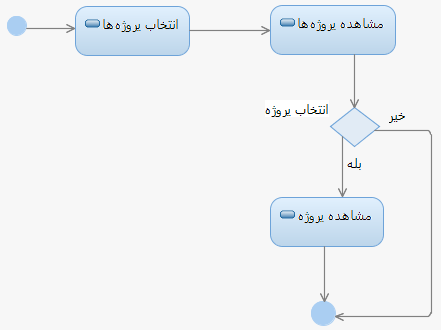
\includegraphics[width=.7\textwidth]{Diagram/3.StateMachine/پروژ‌ه‌ها.png}
\caption{دیاگرام حالت ماشین پروژه‌ها}
\label{fig:sm:پروژه‌ها}
\end{figure}
\begin{figure}[H]
	\centering
	\includegraphics[width=.5\textwidth]{Diagram/4.Collaboration/1.Sequence/پروژه‌ها.png}
	\caption{دیاگرام توالی پروژه‌ها}
	\label{fig:s:پروژه‌ها}
\end{figure}
\begin{figure}[H]
	\centering
	\includegraphics[width=.8\textwidth]{Diagram/4.Collaboration/2.Communication/پروژه‌ها.png}
	\caption{دیاگرام همکار پروژه‌ها}
	\label{fig:c:پروژه‌ها}
\end{figure}
